\documentclass[10pt,compress]{beamer}

\usetheme[usetitleprogressbar]{m}

\usepackage{booktabs,verbatim,math}
\usepackage[scale=2]{ccicons}
\usepackage{tikz}
	\usetikzlibrary{arrows.meta,shapes}
	\everymath{\displaystyle}
	\tikzstyle{na} = [baseline=-.5ex]
	\tikzstyle{ta} = [thick, ->]
	\tikzstyle{every picture}+=[remember picture]
\usepackage{minted}
	\usemintedstyle{trac}
\usepgfplotslibrary{dateplot}

\title{Introduction to Universality}
\subtitle{Phase Transitions in Random Graphs}
\date{July 3, 2015}
\author{Alberto Pezzotta}
%\institute{Institute or miscellaneous information}

% BIBLIOGRAFIA
\usepackage[bibstyle = science,%
			citestyle = authoryear,%
			backend = bibtex]{biblatex}
\bibliography{biblio}
\newcommand{\customcite}[1]{\alert{\citeauthor{#1}, \citeyear{#1}}}
\newcommand{\citeall}[1]{\citeauthor{#1}, \citetitle{#1}, \citeyear{#1}}

\graphicspath{{immagini/}}

\newcommand\tikzmark[1]{%
  \tikz[remember picture,overlay]\node (#1) {};%
}
\newcommand\Connect[3][]{%
\tikz[remember picture,overlay]
  \draw[->,>=latex,#1] (#2.west) -- (#3.east);%
}

\begin{document}

\begin{frame}[plain]
\begin{minipage}[b][\paperheight]{\textwidth}
    \vspace*{2em}
    \begin{figure}
    	\centering
    	
\includegraphics[width=.25\textwidth]{logo_SISSA}
    \end{figure}
\begin{center}
    \ifx\inserttitlegraphic\@empty%
    \else%
    {
    	% actual output of titlegraphic
   	    \usebeamercolor[fg]{titlegraphic}\inserttitlegraphic\par%
    	% measurement and add negative vspace
		\newdimen\logoheight
		\setbox0=\vbox{\inserttitlegraphic}%
		\logoheight=\ht0 \advance\logoheight by \dp0 %
		\vspace*{-\logoheight}%
		\vspace*{-1em}% I don't know why this additional negative space is needed
    }%
    \fi%
    \vfill
    \ifx\inserttitle\@empty%
    \else%
    {%\raggedright
    \linespread{1.0}\usebeamerfont{title}\usebeamercolor[fg]{title}\scshape\MakeLowercase{\inserttitle}\par}%
    \vspace*{0.5em}
    \fi%
    \ifx\insertsubtitle\@empty%
    \else%
    {\usebeamerfont{subtitle}\usebeamercolor[fg]{subtitle}\insertsubtitle\par}%
    \vspace*{0.5em}
    \fi%
    \begin{tikzpicture}\draw[alerted text.fg] (0, 0) -- (\textwidth, 0); \end{tikzpicture} %
    \vspace*{1em}
    \ifx\insertauthor\@empty%
    \else%
    {\usebeamerfont{author}\usebeamercolor[fg]{author}\insertauthor\par}%
    \vspace*{0.25em}
    \fi%
    \ifx\insertdate\@empty%
    \else%
    {\usebeamerfont{date}\usebeamercolor[fg]{date}\insertdate\par}%
    \fi%
    \ifx\insertinstitut\@empty%
    \else%
    \vspace*{3mm}
    {\usebeamerfont{institute}\usebeamercolor[fg]{institute}\insertinstitute\par}%
    \fi%
%    \ifx\insertmainpaper\@empty%
%    \else%
%    \vspace*{1em}
%    {\usebeamerfont{subtitle}\usebeamercolor[fg]{subtitle}\textbf{Pavloff N.}, Phys. Rev. A \textbf{66}, 013610 (2002)\par}
%    \fi
    \vfill
    \vspace*{2em}   	
\end{center}
\end{minipage}
\end{frame}

	
	\section{Universality\newline in phase transitions}
\begin{frame}{An Example from Cold Atoms Physics}
	\vspace*{-3ex}
	\begin{figure}
		\centering
		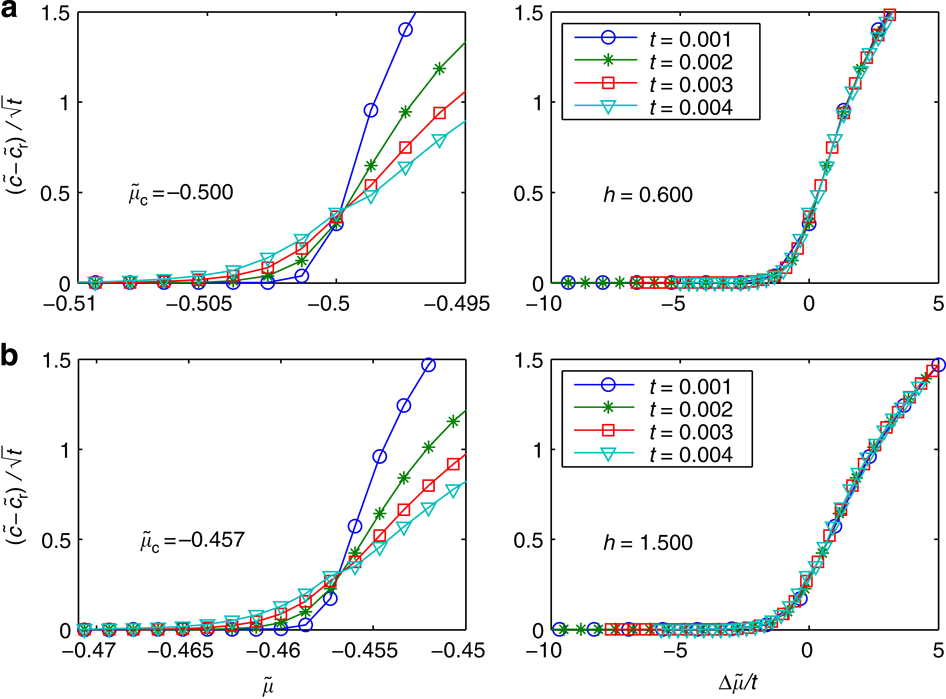
\includegraphics[height=.8\textheight]{contact-universal.png}\\
		(\citeall{contact})
	\end{figure}
\end{frame}
	
	\section{Random Graphs}
\begin{frame}{Why Random Graphs?}
	\begin{center}
		\citeall{newman-netw}
	\end{center}
	\begin{itemize}
		\item<2-> \structure{Model real networks}:
		\begin{itemize}
			\item possibility of tailoring the random graph;
			\item sacrifice some features (\eg clustering coefficient);
			\item interpolating between random graphs and networks (\eg WS and NW small world)
		\end{itemize}
		\item<3-> Make connection with \structure{statistical mechanics}:
		\begin{itemize}
			\item universal properties?
			\item phase transitions $\rightsquigarrow$ giant component
		\end{itemize}
	\end{itemize}
\end{frame}

\begin{frame}{Degree Distribution and \ldots}
	\vspace*{-1.5cm}
	\begin{minipage}[t][0.65\textheight][t]{\textwidth}
	\begin{columns}
		\column{.6\textwidth}
			\begin{figure}
				\centering
				\tiny\def\svgwidth{\columnwidth}
				\only<1>{\input{immagini/graph_plain.pdf_tex}}
				\only<2>{\input{immagini/graph_degrees.pdf_tex}}
				\only<3>{\input{immagini/graph_excess.pdf_tex}}
				\only<4->{\input{immagini/graph_branches.pdf_tex}}
			\end{figure}
		\column{.4\textwidth}
			\begin{center}
				\customcite{nsw-size}
			\end{center}
			\begin{align*}
				\visible<3->{p_k \quad &\rightsquigarrow \quad g_0(z)} \\[1ex]
				\visible<4->{q_k \quad &\rightsquigarrow \quad g_1(z) = \frac{g_0'(z)}{g_0'(1)}} \\[1ex]
				\visible<5->{\rho_t \quad &\rightsquigarrow \quad h_1(z) \visible<7->{= z\,g_1(h_1(z))}} \\[1ex]
				\visible<7->{\pi_s \quad &\rightsquigarrow \quad h_0(z) = z\,g_0(h_1(z))}
			\end{align*}
	\end{columns}
	\end{minipage}
	%
	\begin{minipage}[t][0.35\textheight][t]{\textwidth}
	\vspace*{5ex}
	\begin{center}
		\only<2>{
			$p_k$ = \structure{degree dist.} \\[1ex]
			$g_0(z)$ = \structure{generating function of $p_k$} = $\sum_k p_k\,z^k $}
		\only<3>{
			$q_k$ = \structure{excess degree dist} = $(k+1)p_{k+1} / \av{k}_p $ \\[1ex]
			$g_1(z)$ = \structure{generating function of $q_k$} = $\sum_k q_k\,z^k $}
		\only<4>{
			$\rho_t$ = \structure{branch size dist} \\[1ex]
			$h_1(z)$ = \structure{generating function of $\rho_t$}}
		\only<5->{
			\only<5-6>{$\pi_s$ = \only<5>{\structure{component size dist} =} $\sum_k P(s|k) p_k$}
			\only<6>{; \qquad $h_0(z)$ = \structure{gen. f. of $\pi_s$} = $\sum_s \pi_s\,z^s$}
			\only<7->{{\large\alert{TREE assumption}}}
				\\ \vspace*{-3ex}
				\[ P(s|k) = \sum_{\{t_k\}} \delta(s-1,\, \sum_{m=1}^k t_m) \prod_{m=1}^k \rho_{t_m} \]
			}
	\end{center}
	\end{minipage}
\end{frame}
%
%
\begin{frame}{Giant Component Size}
%	\begin{minipage}[t][0.2\textheight][t]{\textwidth}
		\begin{center}
			$p_k$ normalized to 1: \qquad $g_0(1) = \sum_k p_k = 1$
		\end{center}
		\visible<2->{
		NOT the same for
%		\tikz[baseline]{\node[anchor=north](pi1){
		\alert{$\pi_s$}
%		};}
		, because
		\begin{center}
%			\tikz[topline]{\node[anchor=east](pi2){
				\alert{TREE $\equiv$ SMALL components}
%			};}
		%
		\[
			h_0(1) = 1 - S
		\]
		$S$ = (relative) \structure{size of a giant component}
		\end{center}
		}
%		\begin{tikzpicture}[overlay]
%	        \path[ta] (pi1) edge [bend right=45] (pi2);
%		\end{tikzpicture}
		\visible<3->{
		\[
			\begin{system}
				&h_1(z) = z\,g_1(h_1(z)) \\[1ex]
				&h_0(z) = z\,g_0(h_1(z))
			\end{system}
			\qquad \Rightarrow \qquad
			\begin{system}
				&h_1(1) = \alert{u = g_1(u)} \\[1ex]
				&h_0(1) = \alert{g_0(u) = 1-S}
			\end{system}
		\]
		}
%	\end{minipage}
\end{frame}
%
%
\begin{frame}{Giant Component Size}
	\begin{minipage}[t][0.5\textheight][t]{\textwidth}
		\begin{columns}
			\column{.4\textwidth}
				\[
					\begin{system}
						&u = g_1(u) \\[1ex]
						&S = 1 - g_0(u)
					\end{system}
				\]
				\begin{center}
				\visible<2->{
					\alert{Phase transition}\\[1ex]
					Critical point at $\kappa$ such that
					\[
						g_1'(1) = 1 = \av{k}_\tu{q}
					\]}
				\end{center}
			\column{.6\textwidth}
			\visible<2->{
				\vspace*{-4ex}
				\begin{figure}
					\centering
					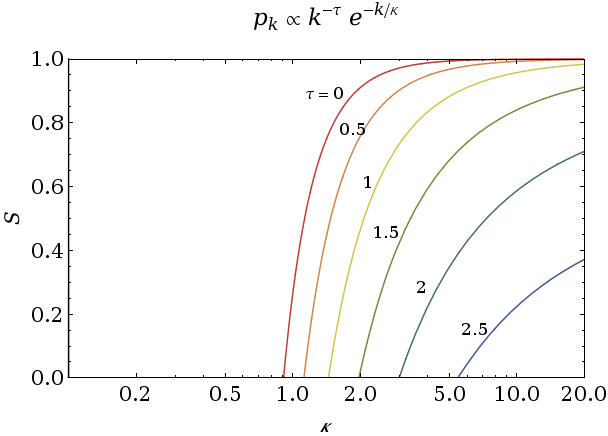
\includegraphics[width=\columnwidth]{phtr_transp}
				\end{figure}}
		\end{columns}
	\end{minipage}
	\visible<3->{\structure{Remarks}:}
	\begin{itemize}
		\item<4-> $\kappa \to \infty \equiv $ \structure{power law} $\rightsquigarrow$ \structure{always} giant component%\\
%			(not true for $\tau \geq 4$; \customcite{scalefree-perc})
		\item<5-> \structure{linear increase} at criticality $\rightsquigarrow$ connection with \structure{percolation} (??)
	\end{itemize}
\end{frame}
%
%
\begin{frame}{A well understood example}
	\vspace*{-4ex}
	\begin{minipage}[t][.4\textheight][t]{\textwidth}
		\structure{Erd\"os--Renyi} random graph $G_{n,p}$ (\customcite{ER}):
		\begin{itemize}
			\item $n$ vertices $\rightsquigarrow$ $n(n-1)/2$ possible edges (links);
			\item each edge drawn with probability $p$ (independently);
	%		\item therefore, the degree has \structure{binomial distribution}
	%			\[
	%				p_k = \binom{n}{k}p^k (1-p)^{n-k} \smc
	%			\]
			\item<2-> in the limit $n \to \infty$, degree $\sim$ \structure{Poisson}, with $c=n p$
				\[
					p_k = \frac{c^{k} e^{-c}}{k!}
					\quad \Rightarrow \quad
					S = 1 - e^{-cS}
				\]
		\end{itemize}
	\end{minipage}
	\begin{columns}
		\column{.5\textwidth}
			\visible<3->{
			\begin{figure}
				\centering
				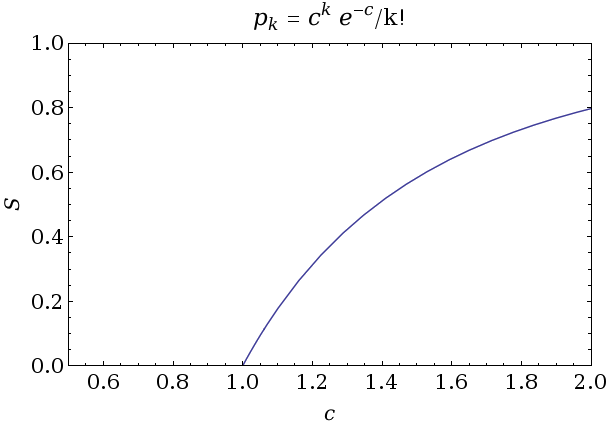
\includegraphics[width=\columnwidth]{ER}
			\end{figure}
			}
		\column{.5\textwidth}
			\visible<4->{
			\structure{Known properties}:
			\begin{itemize}
				\item \structure{equivalency} to \structure{Potts} model (at the level of \structure{Large Deviations}, \customcite{LD-ER});
				\item ph. transition in the universality class of \structure{percolation}, $(q\to 1)$-Potts
			\end{itemize}
			}
	\end{columns}
\end{frame}
%
%
\begin{frame}{Erd\"os--Renyi \& Potts model}
	\vspace*{-2ex}
	$\varphi(G)$ = \# conn. comps in $G$/N; \quad $c$ = average degree
	\begin{align*}
			R_N(\varphi;c) &= \sum_G \mathcal{P}(G)\,\delta(\varphi - \varphi(G)) \sim \exp\{-N r(\varphi; c)\}\\
			\visible<2->{\Rightarrow\  Y_N(q; c) &= \sum_G \mathcal{P}(G)\,q^{N\varphi} = \int_0^1 d\varphi\,R_N(\varphi; c)\,q^{N\varphi} \sim \exp\{-N y(q; c)\}}
	\end{align*}
	\visible<3->{
	\structure{Large deviations}: \structure{rate} and \structure{cumulant generating} functions
	\[
		r(\varphi; c) = \sup_{q\geq 0} \{\varphi\,\ln q - y(q; c)\}
		\quad \leftrightarrow \quad 
		y(q; c) = \sup_{\varphi \in [0,1]} \{\varphi\,\ln q - r(\varphi; c)\}
	\]
	\vspace*{-2ex}
	}
	%
	\visible<4->{
    \begin{tikzpicture}
    	\draw[alerted text.fg] (0, 0) -- (\textwidth, 0);
    \end{tikzpicture} %
	%
	\begin{minipage}[c][.4\textheight][t]{\textwidth}
	\vspace*{1.5ex}
	\structure{Potts model}: $E[\{\sigma_i\}] = - \frac{1}{N}\sum_{i<j} \delta_{\sigma_i \sigma_j}$, \quad where $\sigma_i \in \{0,\ldots q-1\}$\\
	\structure{Partition Function}:\\
		\begin{minipage}[c][.12\textheight][b]{\textwidth}
		$
			Z_N(q; T) \only<4-5,9>{= \sum_{\{\sigma_i\}} e^{(1/NT)\sum_{i<j} \delta_{\sigma_i \sigma_j}}}
					\only<5-7>{= \sum_{\{\sigma_i\}} \prod_{i<j}(1 + w\delta_{\sigma_i \sigma_j})
						\only<6>{\quad \text{(where $w = e^{1/NT} - 1$)}}}
					\only<7-8>{= \sum_G w^{N_e(G)} \prod_{k=0}^{N_e(G)} \delta_{\sigma_{i_k} \sigma_{j_k}}}
					\only<8->{= \sum_G w^{N_e(G)} q^{N\varphi(G)}}
		$
		\end{minipage}
	\end{minipage}
	}
\end{frame}
%
%
\begin{frame}{Erd\"os--Renyi \& Potts model}
	\vspace*{-5ex}
	\[
		w = e^{1/NT} - 1 \equiv \frac{c}{N}
		\quad \Leftrightarrow \quad
		T \equiv \frac{1}{N\,\ln(1+c/N)} \sim \frac{1}{c}
	\]
	\visible<2->{
	Then \structure{equivalence} is \structure{established}:
	\[
		Z_N(q; T=1/c) \simeq e^{Nc/2}\,Y_N(q; c)
		\qquad \text{or} \qquad
		f(q; 1/c) \simeq -\frac{1}{2} - \frac{1}{c} y(q; c)
	\]
	}
	%
	\visible<3->{
	In terms of \structure{fractions} $x(\sigma;\{\sigma_i\}) = \frac{1}{N}\sum_i \delta_{\sigma \sigma_i}$:
	\[
		f(\{x(\sigma)\}_{\sigma=0}^{q-1}; 1/c) = - \sum_{\sigma=0}^{q-1}\left\{\frac{1}{2} x(\sigma)^2 - \frac{1}{c} x(\sigma) \ln x(\sigma) \right\}
	\]
	}
	\visible<4->{
	Equilibrium solution encoding \structure{symmetry breaking}:
	\[
		x(0) = [1+(q-1)s]/q \smc
		\quad
		x(\sigma>0) = (1-s)/q
	\]
	Solutions in the $q\to 1$ limit:
	\begin{description}
		\item[$c\leq 1$]: $s^* = 0$;
		\item[$c>1$]: $s^* = 1 - e^{-cs^*}$ $\rightsquigarrow$ \alert{Erd\"os--Renyi equation}
	\end{description}
	}
\end{frame}


	
	\section{Open Problems}

\begin{frame}{Open Problems}
%	\begin{columns}
%		\column{.7\textwidth}
		\begin{minipage}[t]{.53\textwidth}
			\begin{itemize}
			\setlength\itemsep{3ex}
				\item Connection with \structure{Random Matrix Theory}\visible<2->{, spectra of \vspace*{1ex}}
				\begin{itemize}
				\setlength\itemsep{1ex}
					\item<2-> \structure{adjacency} matrix
						(\customcite{univ-rm};
						\customcite{spectra-srm};
						\customcite{lapl-degree})
					\item<3-> \structure{Laplacian} matrix\\
						(\customcite{ens-aver}).
				\end{itemize}
				\item<4-> Universality of phase transitions in generic degree distribution random graphs (\customcite{cp-cn}; \customcite{scalefree-perc}).
			\end{itemize}		
		\end{minipage}
%		\column{.3\textwidth}
%			\vspace*{-7ex}
		\begin{minipage}[t]{.46\textwidth}
			\vspace*{-2ex}
			\begin{figure}
				\begin{flushright}
					\visible<2->{\hspace*{-5ex}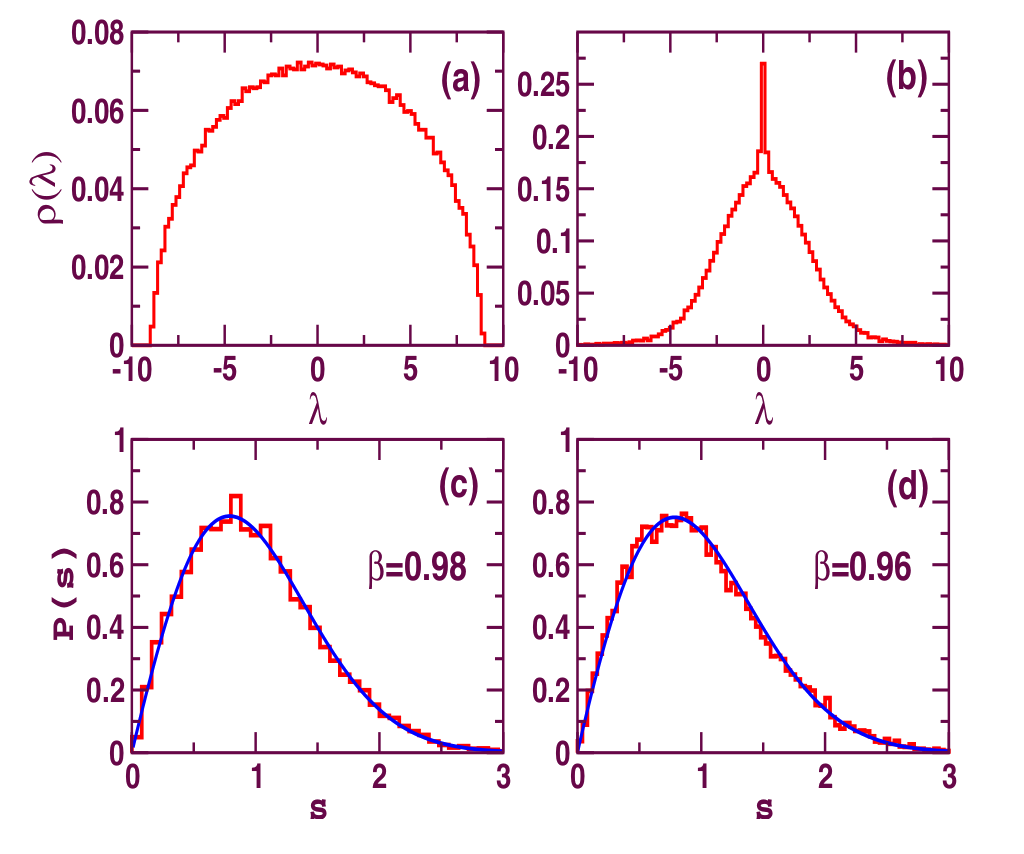
\includegraphics[width=\textwidth]{ER-SF}}\\
%					\hspace*{-5ex}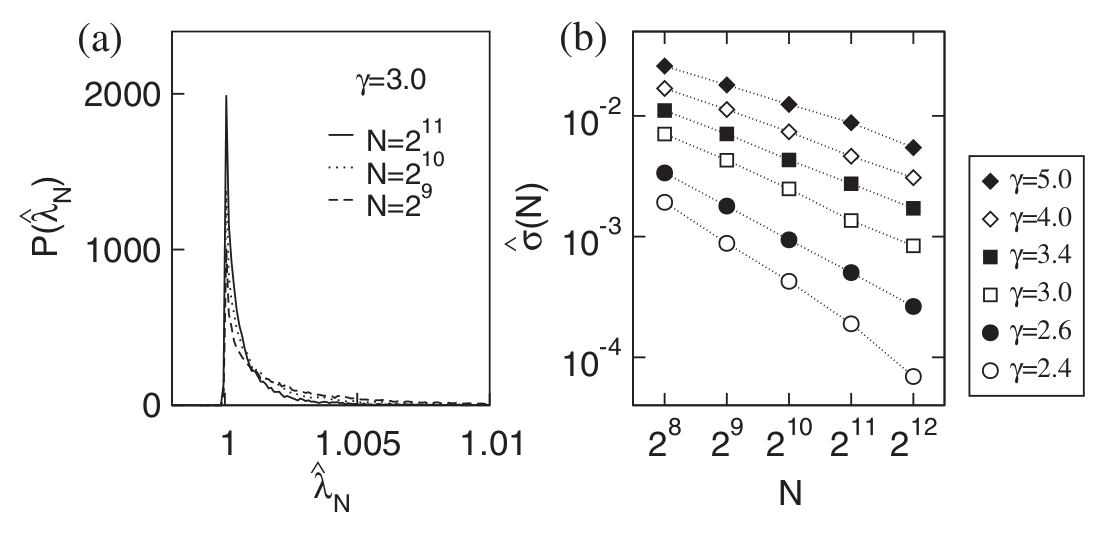
\includegraphics[width=.8\textwidth]{kim-motter}\\
					\visible<4->{\hspace*{-5ex}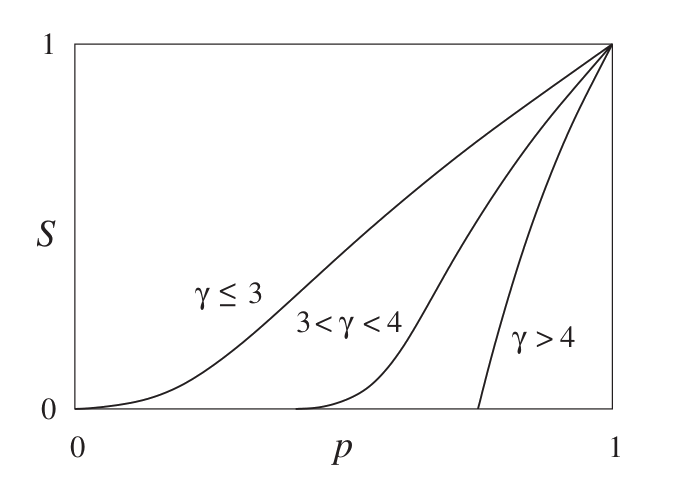
\includegraphics[width=\textwidth]{perc_scale_free}}
				\end{flushright}
			\end{figure}			
		\end{minipage}
%	\end{columns}
\end{frame}


\begin{frame}{References}
	\vspace*{-4ex}
%	\nocite{*}
	\renewcommand*{\bibfont}{\scriptsize}
	\setlength{\bibitemsep}{0.2ex}
	\printbibliography
\end{frame}


\end{document}
